\begin{titlepage}
%\flushleft{\qquad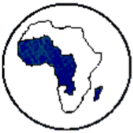
\includegraphics[scale=1.5]{afriq.png}}\qquad\qquad\qquad\qquad\qquad\qquad\qquad\qquad\qquad\qquad\qquad 
\includegraphics[scale=1.5]{imsp.png}

\includegraphics[scale=0.5]{entetememo.png}
%\begin{center}
%\textsc{Université de Porto-Novo} \\ \textsc{The   Abdus Salam  International Centre %for Theoretical Physics}\\ \textsc{\large{Institut de Mathématiques et de Sciences %Physiques}}
%\end{center}
%\begin{center}
%Universit\'e de Porto-Novo \hspace*{\stretch{1}} Institut de %Mathématiques \\ \begin{flushright}et de Sciences Physiques 
%\end{flushright} }

%\end{center}

\parindent=0pt
\definecolor{bordeaux}{rgb}{.5,0,0}\small {} 

\vspace*{\stretch{1}}
\hspace{4cm}
\begin{minipage}{.2\textwidth}\hspace{-2cm}
%\rotatebox{-40}{\LARGE $\textit{  Postulat de Einstein} $} \\
{\vspace{1cm}}
%$\textit{Einstein } \longleftarrow$ \\
%\rotatebox{-40}{\textit{Einstein } $\longleftarrow$} \\\\
% $X\hookrightarrow \mathcal N_(\mu, \sigma)$
\end{minipage}\hspace{-2cm}
\begin{minipage}{.4\textwidth}
\begin{center}
%\includegraphics[scale=0.2]{images/imglivre.png}%
\end{center}
\end{minipage}\hspace{-1cm}
\begin{minipage}{.3\textwidth}\vspace{-3cm}
%\hspace{-1.2cm}\rotatebox{40}{\quad \huge$\displaystyle \int_0^{+\infty} e^{-x^2}\!dx =\frac{\sqrt{\pi}}{2}$}\\
\end{minipage}\\
%\begin{minipage}{.3\textwidth}\vspace{-4cm}
%\textit{int\'egrale de Riemann}\\
%$\longrightarrow$ man can pixe\\
%$\longrightarrow$ man can pixe\\
 %\textit{\'Equations de Maxwell}\\
%$\longrightarrow$ man can pixe\\
%\\
%\end{minipage}\\
\begin{center}
\textsc{\large{\textbf{Rapport scientifique}}} 
\end{center}
\begin{center} Pour l'obtention du Diplôme de Licence spéciale des classes préparatoires option  MPSI spécialité  Mathématiques -- Informatique (MI) \end{center}

\vspace*{\stretch{1}}
\rule{17cm}{3pt}
\begin{center}\bfseries\Large%\Huge
   \textit{\'Etude de quelques familles classiques de polynômes orthogonaux} 
\end{center}
\rule{17cm}{3pt}
\begin{center}\bfseries\Large

\end{center}
    
\[\]
\begin{center}
Présenté par : 
\end{center}
\begin{center}
\textbf{Kenneth ASSOGBA \& Larissa DENAKPO}
\end{center}
\[\]
\[\]
\begin{center}
 Encadré par le : 
 \end{center}
 \begin{center}
  { \bf Professeur Léonard TODJIHOUNDE }
     \end{center}
 
\begin{minipage}{.3\textwidth}

\end{minipage}
\vspace*{7cm}
     
\begin{tikzpicture}[remember picture, overlay]
 \begin{scope}[shift={(current page.south west)},shift={(1,1)},scale=1]
 \shade[ball color=purple,opacity=.6] (0,0) circle (10ex);
 \shade[ball color=purple,opacity=0.5] (1.7,1) circle (5ex);
 \shade[ball color=purple,opacity=.8] (1.5,3) circle (2ex);
 \shade[ball color=cyan,opacity=.5] (-0.5,3) circle (1ex);
 \shade[ball color=orange,opacity=.8] (1,4) circle (1ex);
 \shade[ball color=pink,opacity=.6] (3.5,2.5) circle (2ex);
 \shade[ball color=gray,opacity=.8] (2.5,4.5) circle (4ex);
 \shade[ball color=yellow,opacity=.5] (3,4) circle (3ex);
 \shade[ball color=blue,opacity=.8] (4.5,4.5) circle (3ex);
 \shade[ball color=blue,opacity=.5] (5.1,4.7) circle (2ex);
 \shade[ball color=blue,opacity=.8] (5,6) circle (1.5ex);
 \shade[ball color=blue,opacity=.6] (3.5,5.5) circle (2ex);
 \shade[ball color=blue,opacity=.8] (5,3) circle (1ex);
 \end{scope}
 \end{tikzpicture} 
 
     \begin{center}
     \textbf{Ann\'ee Universitaire:} 2015-2016
     \end{center}
     \vspace*{3cm}

 \end{titlepage}